
\begin{center}
	\begin{adjustbox}{width=7cm, height=12cm, keepaspectratio}
\tikzset{every picture/.style={line width=0.75pt}} %set default line width to 0.75pt        

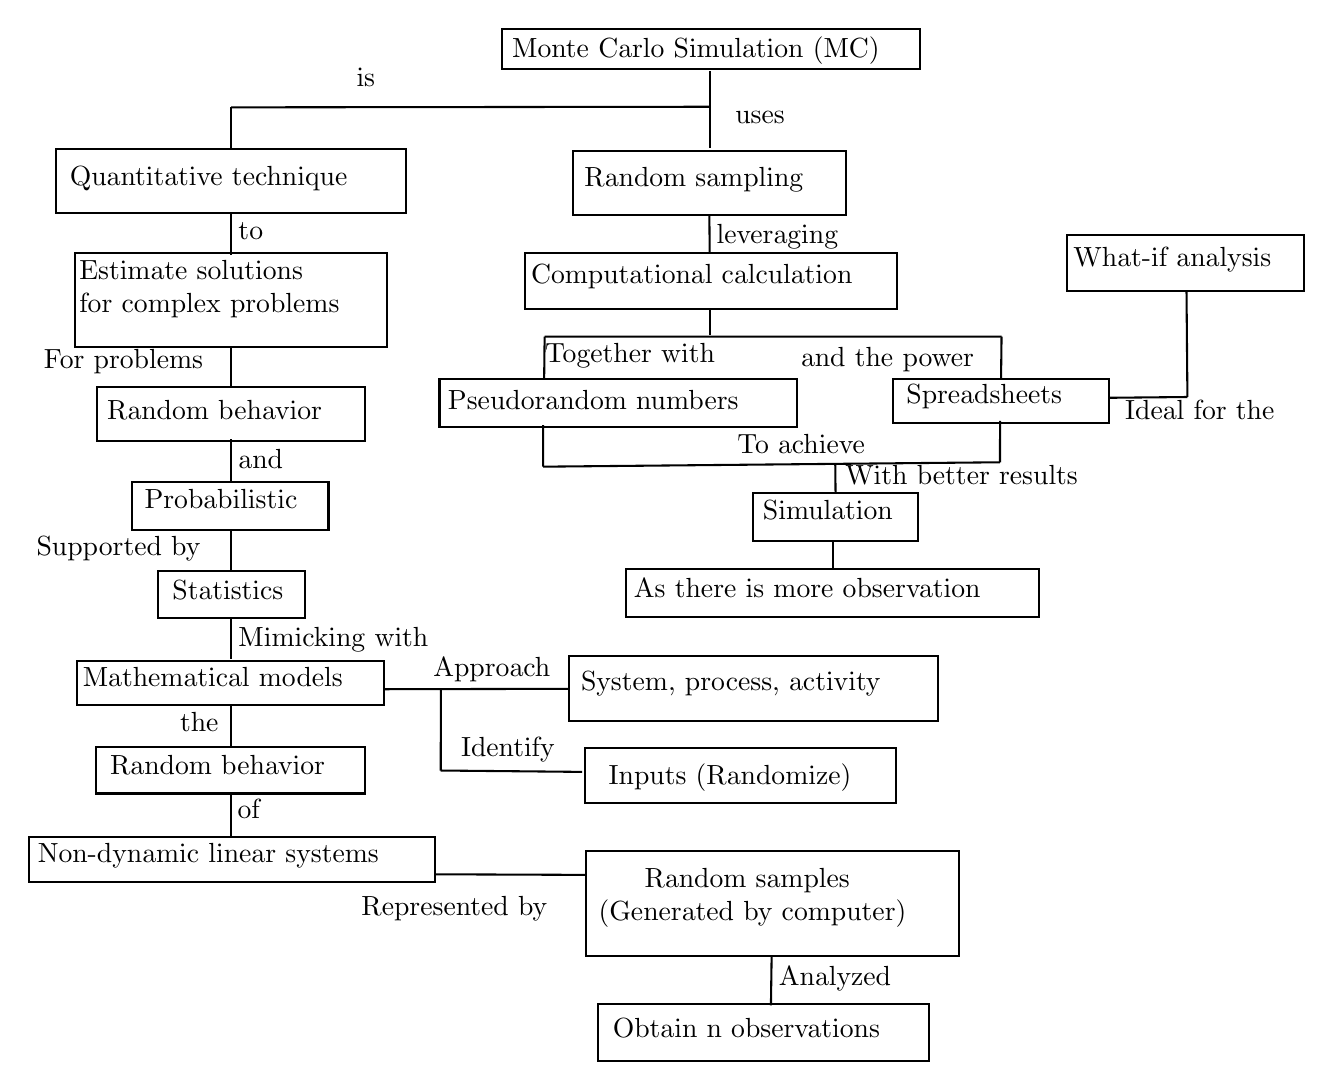
\begin{tikzpicture}[x=0.75pt,y=0.75pt,yscale=-1,xscale=1]
	%uncomment if require: \path (0,533); %set diagram left start at 0, and has height of 533
	
	%Shape: Rectangle [id:dp4215263234124962] 
	\draw   (250.3,22.4) -- (451.7,22.4) -- (451.7,42) -- (250.3,42) -- cycle ;
	
	%Shape: Rectangle [id:dp5605986393419784] 
	\draw   (284.31,81.14) -- (415.64,81.14) -- (415.64,112.05) -- (284.31,112.05) -- cycle ;
	
	%Shape: Rectangle [id:dp6822124988658465] 
	\draw   (35.36,80.38) -- (204.02,80.38) -- (204.02,111.05) -- (35.36,111.05) -- cycle ;
	
	%Straight Lines [id:da24917666653444992] 
	\draw    (119.64,60.29) -- (119.64,80.29) ;
	%Shape: Rectangle [id:dp9161612452597685] 
	\draw   (44.36,130.57) -- (194.5,130.57) -- (194.5,175.71) -- (44.36,175.71) -- cycle ;
	
	%Shape: Rectangle [id:dp8552131257525999] 
	\draw   (54.93,194.86) -- (184.21,194.86) -- (184.21,220.86) -- (54.93,220.86) -- cycle ;
	
	%Shape: Rectangle [id:dp28699352071595885] 
	\draw   (71.79,240.57) -- (166.5,240.57) -- (166.5,264) -- (71.79,264) -- cycle ;
	
	%Shape: Rectangle [id:dp9391104634008505] 
	\draw   (84.36,283.71) -- (155.36,283.71) -- (155.36,306.29) -- (84.36,306.29) -- cycle ;
	
	%Shape: Rectangle [id:dp8058266749569549] 
	\draw   (45.5,326.86) -- (193.07,326.86) -- (193.07,348.29) -- (45.5,348.29) -- cycle ;
	
	%Shape: Rectangle [id:dp6778401923058543] 
	\draw   (54.64,368.29) -- (184.21,368.29) -- (184.21,390.86) -- (54.64,390.86) -- cycle ;
	
	%Shape: Rectangle [id:dp04288092205088323] 
	\draw   (22.07,412) -- (217.64,412) -- (217.64,433.71) -- (22.07,433.71) -- cycle ;
	
	%Straight Lines [id:da42743025398796664] 
	\draw    (119.64,111.29) -- (119.64,131.29) ;
	%Straight Lines [id:da44451579341625] 
	\draw    (119.64,175.29) -- (119.64,195.29) ;
	%Straight Lines [id:da2952815700269025] 
	\draw    (119.64,220.29) -- (119.64,240.29) ;
	%Straight Lines [id:da23583722394609818] 
	\draw    (119.64,264.29) -- (119.64,284.29) ;
	%Straight Lines [id:da8623849950040359] 
	\draw    (119.64,306.29) -- (119.64,326.29) ;
	%Straight Lines [id:da20115540357810247] 
	\draw    (119.64,348.29) -- (119.64,368.29) ;
	%Straight Lines [id:da5844455334116092] 
	\draw    (119.64,391.29) -- (119.64,411.29) ;
	
	%Straight Lines [id:da3223201886985534] 
	\draw    (350.21,42.86) -- (350.21,80) ;
	%Straight Lines [id:da5360135696422039] 
	\draw    (119.64,60.29) -- (350.5,60) ;
	
	%Straight Lines [id:da04617213993490532] 
	\draw    (350,112.21) -- (350.17,130.54) ;
	%Shape: Rectangle [id:dp19377800699756875] 
	\draw   (261.11,130.29) -- (440.33,130.29) -- (440.33,157.62) -- (261.11,157.62) -- cycle ;
	
	%Shape: Rectangle [id:dp9948484136770976] 
	\draw   (220,191.18) -- (392.11,191.18) -- (392.11,214.29) -- (220,214.29) -- cycle ;
	
	%Shape: Rectangle [id:dp3384676720419708] 
	\draw   (438.44,191.18) -- (542.56,191.18) -- (542.56,212.51) -- (438.44,212.51) -- cycle ;
	
	%Shape: Rectangle [id:dp27123736378500474] 
	\draw   (370.89,246.07) -- (450.56,246.07) -- (450.56,269.18) -- (370.89,269.18) -- cycle ;
	
	%Shape: Rectangle [id:dp38853819472250084] 
	\draw   (309.78,282.73) -- (509,282.73) -- (509,305.62) -- (309.78,305.62) -- cycle ;
	
	%Straight Lines [id:da014310810654853512] 
	\draw    (350.22,157.21) -- (350.22,170.14) ;
	%Straight Lines [id:da4776425539155458] 
	\draw    (270.64,170.78) -- (270.41,190.77) ;
	%Straight Lines [id:da4769047517207039] 
	\draw    (270.64,170.78) -- (490.78,170.73) ;
	%Straight Lines [id:da7827579715275725] 
	\draw    (490.78,170.73) -- (490.54,190.72) ;
	%Straight Lines [id:da7330155577088908] 
	\draw    (410.8,245.61) -- (410.67,232.68) ;
	%Straight Lines [id:da8509011957588517] 
	\draw    (490.02,231.29) -- (490.07,211.3) ;
	%Straight Lines [id:da5588878306465803] 
	\draw    (490.02,231.29) -- (269.9,233.41) ;
	%Straight Lines [id:da6769845464898216] 
	\draw    (269.9,233.41) -- (269.94,213.42) ;
	
	%Straight Lines [id:da6666639120422786] 
	\draw    (409.78,269.65) -- (409.78,282.58) ;
	%Shape: Rectangle [id:dp8402670006761139] 
	\draw   (522.44,121.62) -- (636.56,121.62) -- (636.56,148.84) -- (522.44,148.84) -- cycle ;
	
	%Straight Lines [id:da5295493181430606] 
	\draw    (580.33,199.84) -- (542.67,200.22) ;
	%Straight Lines [id:da9855214298674604] 
	\draw    (579.89,148.51) -- (580.33,199.84) ;
	
	%Shape: Rectangle [id:dp5002143400150245] 
	\draw   (282.33,324.46) -- (460,324.46) -- (460,355.8) -- (282.33,355.8) -- cycle ;
	
	%Shape: Rectangle [id:dp35257179506306247] 
	\draw   (290,369.13) -- (440,369.13) -- (440,395.46) -- (290,395.46) -- cycle ;
	
	%Shape: Rectangle [id:dp4882311664786725] 
	\draw   (290.43,418.65) -- (470.1,418.65) -- (470.1,469.32) -- (290.43,469.32) -- cycle ;
	
	%Shape: Rectangle [id:dp0619736638622812] 
	\draw   (296.33,492.46) -- (456,492.46) -- (456,519.8) -- (296.33,519.8) -- cycle ;
	
	%Straight Lines [id:da8550561367501606] 
	\draw    (193.33,340.63) -- (281.86,340.44) ;
	%Straight Lines [id:da39616791435448273] 
	\draw    (220.57,379.8) -- (288.67,380.46) ;
	%Straight Lines [id:da11167548719220122] 
	\draw    (220.67,340.55) -- (220.57,379.8) ;
	%Straight Lines [id:da16209257991496884] 
	\draw    (217.71,429.8) -- (290.71,430.08) ;
	%Straight Lines [id:da46148840186933593] 
	\draw    (380,469.55) -- (379.67,492.94) ;
	
	% Text Node
	\draw (253.5,25) node [anchor=north west][inner sep=0.75pt]   [align=left] {Monte Carlo Simulation (MC)};
	% Text Node
	\draw (288.31,87.79) node [anchor=north west][inner sep=0.75pt]   [align=left] {Random sampling};
	% Text Node
	\draw (40.36,87.38) node [anchor=north west][inner sep=0.75pt]   [align=left] {Quantitative technique};
	% Text Node
	\draw (44.93,132.43) node [anchor=north west][inner sep=0.75pt]   [align=left] {Estimate solutions \\for complex problems};
	% Text Node
	\draw (58.36,199.86) node [anchor=north west][inner sep=0.75pt]   [align=left] {Random behavior};
	% Text Node
	\draw (76.36,242.86) node [anchor=north west][inner sep=0.75pt]   [align=left] {Probabilistic};
	% Text Node
	\draw (89.79,286.86) node [anchor=north west][inner sep=0.75pt]   [align=left] {Statistics};
	% Text Node
	\draw (46.64,328.43) node [anchor=north west][inner sep=0.75pt]   [align=left] {Mathematical models};
	% Text Node
	\draw (59.79,370.86) node [anchor=north west][inner sep=0.75pt]   [align=left] {Random behavior};
	% Text Node
	\draw (24.93,413.57) node [anchor=north west][inner sep=0.75pt]   [align=left] {Non-dynamic linear systems};
	% Text Node
	\draw (178.5,40) node [anchor=north west][inner sep=0.75pt]   [align=left] {is};
	% Text Node
	\draw (361,61) node [anchor=north west][inner sep=0.75pt]   [align=left] {uses};
	% Text Node
	\draw (121.64,114.29) node [anchor=north west][inner sep=0.75pt]   [align=left] {to};
	% Text Node
	\draw (27.93,175.21) node [anchor=north west][inner sep=0.75pt]   [align=left] {For problems};
	% Text Node
	\draw (121.64,223.29) node [anchor=north west][inner sep=0.75pt]   [align=left] {and};
	% Text Node
	\draw (24.36,265.29) node [anchor=north west][inner sep=0.75pt]   [align=left] {Supported by};
	% Text Node
	\draw (121.64,309.29) node [anchor=north west][inner sep=0.75pt]   [align=left] {Mimicking with};
	% Text Node
	\draw (93.5,350.43) node [anchor=north west][inner sep=0.75pt]   [align=left] {the};
	% Text Node
	\draw (121.21,392.14) node [anchor=north west][inner sep=0.75pt]   [align=left] {of};
	% Text Node
	\draw (262.61,134.61) node [anchor=north west][inner sep=0.75pt]   [align=left] {Computational calculation};
	% Text Node
	\draw (222.56,195.22) node [anchor=north west][inner sep=0.75pt]   [align=left] {Pseudorandom numbers};
	% Text Node
	\draw (374.33,247.94) node [anchor=north west][inner sep=0.75pt]   [align=left] {Simulation};
	% Text Node
	\draw (312.17,285.67) node [anchor=north west][inner sep=0.75pt]   [align=left] {As there is more observation};
	% Text Node
	\draw (443.44,192.44) node [anchor=north west][inner sep=0.75pt]   [align=left] {Spreadsheets};
	% Text Node
	\draw (523.94,126.06) node [anchor=north west][inner sep=0.75pt]   [align=left] {What-if analysis};
	% Text Node
	\draw (286.67,330.62) node [anchor=north west][inner sep=0.75pt]   [align=left] {System, process, activity};
	% Text Node
	\draw (300,374.95) node [anchor=north west][inner sep=0.75pt]   [align=left] {Inputs (Randomize)};
	% Text Node
	\draw (295.1,425.48) node [anchor=north west][inner sep=0.75pt]   [align=left] { \ \ \ \ \ Random samples \\(Generated by computer)};
	% Text Node
	\draw (302,497.62) node [anchor=north west][inner sep=0.75pt]   [align=left] {Obtain n observations};
	% Text Node
	\draw (352,115.21) node [anchor=north west][inner sep=0.75pt]   [align=left] {leveraging};
	% Text Node
	\draw (269.33,172.67) node [anchor=north west][inner sep=0.75pt]   [align=left] {Together with};
	% Text Node
	\draw (392.67,174.33) node [anchor=north west][inner sep=0.75pt]   [align=left] {and the power};
	% Text Node
	\draw (362,216.33) node [anchor=north west][inner sep=0.75pt]   [align=left] {To achieve};
	% Text Node
	\draw (414,231.33) node [anchor=north west][inner sep=0.75pt]   [align=left] {With better results};
	% Text Node
	\draw (215.52,323.76) node [anchor=north west][inner sep=0.75pt]   [align=left] {Approach};
	% Text Node
	\draw (228.86,362.16) node [anchor=north west][inner sep=0.75pt]   [align=left] {Identify};
	% Text Node
	\draw (180.86,438.87) node [anchor=north west][inner sep=0.75pt]   [align=left] {Represented by};
	% Text Node
	\draw (382,472.55) node [anchor=north west][inner sep=0.75pt]   [align=left] {Analyzed};
	% Text Node
	\draw (548.86,199.73) node [anchor=north west][inner sep=0.75pt]   [align=left] {Ideal for the};
	
	
\end{tikzpicture}
\end{adjustbox}
\end{center}
